\documentclass[oneside]{VUMIFPSkursinis}
\usepackage{algorithmicx}
\usepackage{algorithm}
\usepackage{algpseudocode}
\usepackage{amsfonts}
\usepackage{float}
\usepackage{amsmath}
\usepackage{bm}
\usepackage{caption}
\usepackage{color}
\usepackage{float}
\usepackage{graphicx}
\usepackage{listings}
\usepackage{subfig}
\usepackage{tabularx}
\usepackage{wrapfig}
\newcolumntype{P}[1]{>{\centering\arraybackslash}p{#1}}
\usepackage[%  
    colorlinks=true,
    linkcolor=black
]{hyperref}
\university{Vilniaus universitetas}
\faculty{Matematikos ir informatikos fakultetas}
\department{Programų sistemų katedra}
\papertype{}
\title{Virtualios ir realios mašinos modelis}
\titleineng{Virtual and real machine model}
\status{2 kurso 3 grupės studentai}
\author{Matas Savickis}
\secondauthor{Justas Tvarijonas}  
\thirdauthor{Greta Pyrantaitė}   
\supervisor{Mantas Grubliauskas Lekt.}
\date{Vilnius – \the\year}


\bibliography{bibliografija}

\begin{document}
\maketitle
\tableofcontents

\section{Reali mašina}
\begin{figure}[H]
		\centering	
	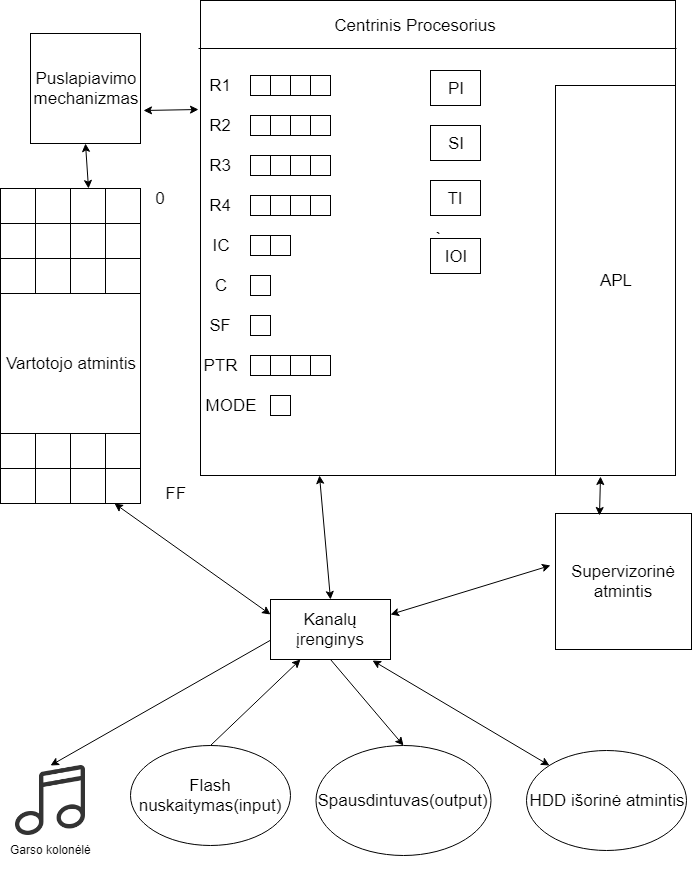
\includegraphics[width=18cm,height=20cm,keepaspectratio]{RealiMasina.png}
	\caption{Reali mašina}
	\label{fig:Reali mašina}
\end{figure}

\pagebreak

\subsection{Techninės įrangos elementai sudarantys realią mašiną}
\begin{itemize}
	\item{Centrinis procesorius}
	\item{Vartotojo atmintis}
	\item{Supervizorinė atmintis}
	\item{Išorinė atmintis}
	\item{Duomenų perdavimo kanalai}
	\item{Įvedimo įrenginys - flash atmintinis}
	\item{Išvedimo įrenginys - spausdintuvas}
	\item{Puslapiavimo mechanizmas}
\end{itemize}

\subsection{Centrinis procesorius}
	Centrinio procesoriaus paskirtis yra skaityti komandas iš atminties ir jas interpretuoti. Procesorius gali dirbti dviem rėžimais - supervizoriaus ir vartotojo. Supervizoriaus rėžime komandos yra apdorojamos aukšto lygio procesoriaus. Komandos vykdomos supervizoriaus režime yra skirtos operacinės sistemos funkcionavimui palaikyti. Procesorius persijungia į šį rėžimą pertaukimais arba sisteminiais kreipiniais.
\subsection{Procesoriaus registrai}
\begin{itemize}
	\item{R1, R2, R3, R4 - 4 baitų bendros paskirties registrai}
	\item{DS - registras rodantis duomenų segmento adresą}
	\item{CS - registras rodantis kodo segmento adresą}
	\item{IC - 2 baitų komandų skaitiklis}
	\item{C - 1 baito loginis registras (TRUE arba FALSE)}
	\item{SF - 1 baito požymių registras CF OF XX XXXZF - carry flag, overflow flag, zero flag}
	\item{PTR - 4 baitų puslapių lentelės registras(naudojamo puslapių lentelės numeris)}
	\item{MODE - registras, kurio reikšmė nusako procesoriaus darbo režimą(supervizorinis, vartotojo)}
	\item{PI - programinių pertraukimų registras}
	\item{SI - supervizorinių pertraukimų registras}
	\item{TI - taimerio registras}
	\item{CHST[1]...CHST[3] - kanalų būsenos registrai }
	\item{IOI - 2 baitų įvedimo ir išvedimo pertraukimų registras}
\end{itemize}

\subsection{Atmintys}
Pagrindinę realios mašinos atmintį dalinasi vartotojo ir supervizorinė atmintis. Kaskart sukuriant naują virtualią mašiną panaudojama dalis realios mašinos atminties. Atminties dydis 16 blokų po 16 žodžių. Žodžio ilgis 4 baitai. Supervizorinę atmintį naudoja aukšto lygio procesorius, tačiau šios atminties savo rašomoje programoje nenaudosim. Taip pat yra išorinė atmintis kietojo disko pavidalu.

\subsection{I/O}
Komandų įvedimui naudojamas ,,flash atmintinių" nuskaitymo įrenginys. Išvedimui naudojamas spausdintuvas.

\subsection{Puslapiavimo mechanizmas}
Puslapiavimo mechanizmas yra metodas skirtas virtualios atminties adreso parodymui į realios atminties adresą. Kiekvienai virtualiai mašinai skiriama 4 atminties blokai. Paskutinis lentelės blokas yra užpildomas realiais adresais. Naudojamas PTR(4 baitų a0,a1,a2,a3) registras kuriame laikomas puslapių lentelės bloko realūs adresai. Pagal a2 ir a3 baitus surandame bloką. Pagal virtualaus adreso x1 ir x2 yra nustatomas puslapis. Bloko adresas kur x1 randamas [4*(4*a2 a3)+x1], o prie bloko adreso pridėjus x2 gauname virtualų adresą: 4*[4*(4*a2 a3)+x1]x2.

\subsection{Duomenų perdavimo kanalai}
Skirti I/O ir atminties valdymui. Modelyje egzistuoja trys kanalai iš kurie kiekvienas atsakingas už skirtingus dalykus. Kanale vyksta arba rašymas arba skaitymas ir pabaigęs darbąą jis informuoja centrinį procesorių ir sukelia pertraukimą padidindamas IOI registro reikšmę. Kanalų būsenos yra saugomos CHST[1]...CHST[3] registruose.





\section{Virtuali mašina}

\subsection{Funkcija}
Virtuali mašina yra skirta paslepti realios mašinos sudėtingumą ir suteikti vartotojui instrukcijų sąrašą su kuriuo jis galėtų dirbti. Todėl operacinės sistemos paskirtis ir yra paslėpti realią mašiną ir duoti mums virtualią. Virtuali mašina taip pat suteikia darbų pasidalijimą kurio dėk galima paleisti kelias virtualias mašinas ir tokiu būdu ant kiekvienos iš jų atlikti skirtingas užduotis.

 \subsection{Modeliuojamos virtualios mašinos loginių komponentų aprašymas}
	\subsubsection{Atmintis}
	\begin{figure}[H]
		\centering	
	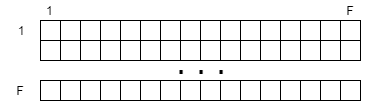
\includegraphics[width=18cm,height=20cm,keepaspectratio]{VMAtmintis.png}
	\caption{Virtualios mašinos atmintis}
	\label{fig:Virtualios mašinos atmintis}
\end{figure}

	Virtualios mašinos atmintis susideda iš 4 blokų po 16 žodžių iš viso 64 žodžiai po 4 baitus arba 32 bitus. Pirmi du atminties blokai bus paskirti duomenų segmentui(DS), o paskutiniai du blokai kodo segmentui(CS). Norint pasinaudoti puslapiavimo mechanizmu pirmas blokas bus išskiriamas surašyti realiems adresams. Naudosime registrą PTR(4 baitai a0 a1 a2 a3) kuriame laikomas puslapių lentelės bloko realūs adresai. Per a2 ir a3 surandame bloką. Pagal x1 ir x2 nustatomas puslapis. Bloko adresas, kur yra x1 randamas pagal formulę [4*(4*a2 a3)+x1]x2, o prie bloko adreso pridėjus x2 gauname vistualų adresą 4*[4*(4*a2 a3)+x1]x2 .Efektyviai naudotis Virtualia atmintimi įvesime du papildomus registus DS ir CS. DS registro reikšmė bus rodyklė į duomenų segmento atmintį, o CS reišmė rodyklė į kodo segmento atmintė.

	\subsubsection{Procesorius}
\begin{figure}[H]
		\centering	
	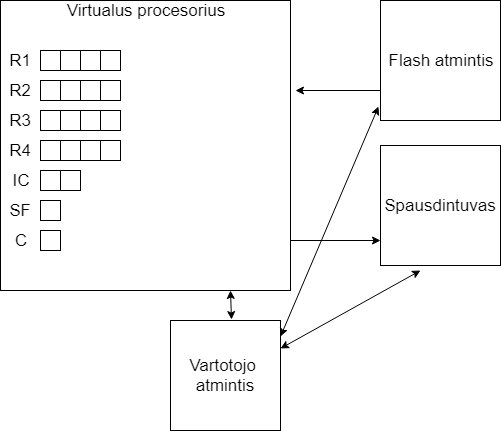
\includegraphics[width=18cm,height=20cm,keepaspectratio]{VMProcesorius.png}
	\caption{Virtualios mašinos procesorius}
	\label{fig:Virtualios mašinos procesorius}
\end{figure}
Registrai:
\begin{itemize}
	\item{R1...R4 - Bendros paskirties registrai}
	\item{IC - komandos skaitliukas, rodo sekančios komandos adresą }
	\item{SF - status flagas rodantis programos būseną}
	\item{C - loginis registras(TRUE arba FALSE)}
	\item{DS - rodo į duomenų segmentą atmintyje}
	\item{CS - rodo į kodo segmentą atmintyje}
\end{itemize}
	\subsubsection{Virtualios mašinos komandų sistema}
Kiekvieną virtualios mašinos komandą sudaro 4B, tačiau priklausomai nuo komandos ne visi
baitai turi būti užimti – jie gali būti ir tušti.
Komandos:
\begin{enumerate}
\item Duomenų persiuntimui iš atminties į registrus ir atvirkščiai:
\begin{enumerate}
\item  LR – Load Register – iš atminties baito x1x2 persiunčia į registrą R:
LR x1x2 =) R:=[x1x2];
\item SR – Save Register – iš registro R persiunčia į atminties baitą x1x2:
SR x1x2 =) [x1x2]:=R;
\end{enumerate}
\item Duomenų sukeitimui tarp registrų:
\begin{enumerate}
\item RR – sukeičia registro R ir R2 reikšmes:
RR =) R:=R+R2, R2=R-R2, R=R-R2;
\end{enumerate}
\item Aritmetinės komandos:
\begin{enumerate}
\item AD – suma – prie esamos registro R reikšmės prideda reikšmę esančią x1x2 atminties
baite, rezultatas patalpinamas registre R:
AD x1x2 =) r1:=r1+[x1x2];
\item SB – atimtis – iš esamos registro R reikšmės atimama reikšmė esanti x1x2 atminties
baite, rezultatas patalpinamas registre R:
SB x1x2 =) r1:=r1-[x1x2];
\item CR – palyginimas – esamą registro R reikšmė yra lyginama su reikšme esančią x1x2
atminties baite, rezultatas patalpinamas registre C:
CR x1x2 =)
if r1>[x1x2] then cf:=0, zf:=0;
if r1=[x1x2] then zf:=1;
if r1<[x1x2] then cf:=1;
\item MU x1x2 – daugyba, r1 =r1* [x1x2].
\item DI x1x2 – dalyba, r1=r1/[x1x2] , r2=r1\%[x1x2].
\end{enumerate}
\item Valdymo perdavimo:
\begin{enumerate}
\item JU – besąlyginio valdymo perdavimas – valdymas perduodamas adresu 16*x1+x2:
JU x1x2 =) IC:=16*x1+x2;
\item JG – sąlyginio valdymo perdavimas (jeigu daugiau) – valdymas perduodamas jeigu
C=0, valdymas perduodamas adresu 16*x1+x2:
JG x1x2 =) If C=0 then IC:= 16*x1+x2;
\item JE – sąlyginio valdymo perdavimas (jeigu lygu) – valdymas perduodamas jeigu C=1,
valdymas perduodamas adresu 16*x1+x2:
JE x1x2 =) If C=1 then IC:= 16*x1+x2;
\item JL – sąlyginio valdymo perdavimas (jeigu mažiau) – valdymas perduodamas jeigu
C=2, valdymas perduodamas adresu 16*x1+x2:
JL x1x2 =) If C=2 then IC:= 16*x1+x2;
\end{enumerate}
\item Darbo su bendra atminties sritimi (prieinama visoms vartotojo programoms; komandos
leidžia į ją rašyti ir skaityti; sritis apsaugoma semaforais):
\begin{enumerate}
\item SM – registro R įrašymas į bendrąją atmintį:
SM x1x2 =)[16*[16*(16*a2 a3)+x1]x2]:=R (pagal puslapiavimo mechanizmą);
\item LM – iš bendrosios atminties įrašomas žodis į registrą R:
LM x1x2 =) R:= [16*[16*(16*a2 a3)+x1]x2] (pagal puslapiavimo mechanizmą);
\end{enumerate}
\item Programos pabaigos:
\begin{enumerate}
\item HALT – programos pabaigos komanda.
\end{enumerate}
\item Įvedimo/Išvedimo:
\begin{enumerate}
\item GD – įvedimas – iš įvedimo srauto paima 1 žodžio srautą ir jį įveda į atmintį
pradedant atminties baitu 16*x1+x2:
GD x1x2
\item PD – išvedimas – iš atminties, pradedant atminties baitu 16*x1+x2 paima 1 žodžio
srautą ir jį išveda į ekraną:
PD x1x2
\end{enumerate}
\item Loginės:
\begin{enumerate}
\item AND – r1 := r1 and r2
\item XOR – r1 := r1 xor r2
\item OR - r1 := r1 or r2.
\item NOT - r1 := not r1.
\end{enumerate}
\item Operavimo failais:
\begin{enumerate}
\item FC - uždaromas failas, kurio handleris yra r1.
\item FO x1x2 – atidaromas [x1x2[ pavadinimo failas. Handleris įrašomas į r1.
\item FR x1x2 – r1 – handleris, r2 – adresas, iš kur skaitome. 16*x1+x2 – virtualios atminties
vieta, į kurią įrašysime.
\item FW x1x2 – handleris, r2 – adresas, iš kur skaitome. 16*x1+x2 – virtualios atminties
vieta, iš kurios rašysime į failą.
\item FD – ištrinamas failas, kurio handleris yra r1.
\end{enumerate}
\end{enumerate}
\subsection{Virtualios mašinos bendravimo su įvedimo/išvedimo įrenginiais mechanizmo aprašymas.}
VM duomenis skaito iš flash atminties (realizuotos failu kietajame diske), o rezultatą išveda spausdintuvas. Įvedimą/išvedimą kontroliuoja kanalų įrenginys.
\subsection{Virtualios mašinos interpretuojamojo ar kompiliuojamo vykdomojo failo išeities teksto formatas.}
VM modelio įvedimo įrenginiui pateikiamas programos failas turi būti tokios struktūros: \newline
DATASEG\newline
.\newline
.\newline
.\newline
CODESEG\newline
.\newline
.\newline
.\newline
HALT\newline
Atmintis yra išdėstyta nuosekliai: 128 žodžiai skirti DATASEG (nuo 0 iki 127) ir 128 žodžiai\newline
CODESEG (nuo 128 iki 255).\newline
Duomenų segmento apraše galimi tokie atvejai:\newline
DW - Išskiriamas vienas tuščias žodis skaitinei reikšmei.\newline
DW X - Išskiriamas vienas žodis ir į jį talpinama nurodyta skaitinė reikšmė.\newline
DB ssss - Išskiriamas vienas žodis ir į jį talpinami keturi nurodyti simboliai.\newline
DB nnnn - Tai rezervuota simbolinė konstanta, reiškianti ?????????? papildyti !!!!!!!.\newline
Programa apskaičiuoja reiškinio „100 + 20 – 80“ reikšmę, bei ją išveda į ekraną.\newline
000 | DATA\newline
001 | 100\newline
002 | 20\newline
003 | 80\newline
004 | Rezu\newline
005 | ltat\newline
009 | as y\newline
00A | ra:\newline
080 | CODE\newline
081 | LR 01\newline
082 | AD 02\newline
083 | SB 03\newline
084 | PD 04\newline
085 | PD 05\newline
086 | PD 06\newline
087 | PD 07\newline
088 | SR 10\newline
089 | PD 10\newline
08A | HALT\newline
0FF |\newline
	\subsection{Modeliuojamos virtualios mašinos loginių komponentų sąryšio su realios mašinos techninės įrangos komponentais aprašymas.}
	Virtualiai mašinai atliekant komandas gali kilti pertraukimai. Jie apdorojami tik tada kai VM
baigia vykdyti komandą.Tuomet reali mašina persijungia iš vartotojo režimo į supervizorinį.\newline
Įvedimo/ Išvedimo veiksmas atliekamas supervizoriniu rėžimu, tam naudojama iniciavimo
operacija StarIO – kuria nustatomi kanalai, jų panaudojimas ir tikrinamas užimtumas.\newline
Norint iš supervizorinio rėžimo į vartotojo rėžimą darbo pratęsimui virtualioje mašinoje
reikalinga pakrauti būsena tam naudojama operacija Slave(plr,c,r,ic) – kur registrų panaudojimas
sutampa su realios mašinos.
	\section{Virtuali mašina operacinės sistemos kontekste}
	Operacinei sistemai turi būti pateikiamas užduočių rinkinys (programa). Tam reikalinga specifinė užduočių pateikimo kalba. Kiekviena užduotis suformuojama kaip failas. Užduotis sudaryta iš pateikiamų duomenų ir rezultatų. Vykdant užduotį ji yra išskaidoma į dalis: užduotis saugoma išorinėje atmintyje, kai ji paruošta vykdymui. Užduotis tiesioginės sąveikos su fiziniais įrenginiais neturi, tik su virtualiais.


\end{document}